%
% ─── CAPITULO 8: VISUALIZACION DE FRACTALES 3D ──────────────────────────────────
%

En el capítulo \ref{chap:fractales-2D} introdujimos técnicas y código necesario para poder visualizar conjuntos de Julia y conjuntos de Mandelbrot 2-dimensionales en un canvas utilizando WebGL, todo ello apoyado en la teoría explicada en el capítulo \ref{chap:Julia-Mandelbrot}. Sin embargo, el objetivo de éste y de los tres capítulos anteriores es aplicar técnicas avanzadas de renderizado para poder visualizar fractales en tres dimensiones. Recordamos que explicamos en la introducción del capítulo \ref{chap:ray-tracing} que la mejor forma de renderizar fractales 3D es utilizando la técnica de `Ray Tracing', que en dicho capítulo explicamos con detalle. A pesar de ello y de conseguir escenas con varios objetos, materiales y movimientos de cámara no visualizamos nada lejanamente parecido a un fractal. Será en este capítulo en el que aprovecharemos toda la infraestructura y todo el código implementado hasta el momento en el `ray-tracer' del capítulo \ref{chap:ray-tracing} para graficar fractales tridimensionales.

Para ello, antes aún debemos asentar una serie de conceptos que son los que nos ayudarán a cumplir nuestro objetivo: el algoritmo \textit{Ray-Marching} y las conocidas como \textit{Signed Distance Functions} (SDFs). Con estos dos elementos combinados conseguiremos ver hermosas figuras fractales.

\section{El algoritmo Ray-Marching}
\label{section:ray-arching}

Hasta ahora siempre hemos calculado las intersecciones rayo-esfera de manera totalmente analítica, ya que es muy sencillo describir una esfera o un plano mediante una ecuación y solucionar esta ecuación en $t$, como vimos en las secciones \ref{subsection:esfera} y \ref{subsection:plano}. Sin embargo, no es tan sencillo encontrar ecuaciones que describan la superficie de los fractales. Es por esto que necesitamos otra manera de encontrar las intersecciones rayo-superficie. Aunque no tengamos una forma de calcular analíticamente la intersección, si contamos con funciones que nos estiman, fijado un punto, a qué distancia se halla este punto del fractal mediante una cota, las conocidas como SDFs (sección \ref{section:SDFs}). De igual manera, si fijamos un punto $p\in\R^3$, podemos calcular a qué distancia se encuentra dicho punto de una esfera o de un plano. 

El algoritmo \textit{Ray-Marching}, también conocido como \textit{Sphere-Tracing} es una técnica utilizada en Ray-Tracing y que se basa en estimar la distancia a la que se encuentra un punto de cada una de las superficies que componen la escena y avanzar en el rayo una distancia correspondiente a la mínima de estas distancias, pues se tiene la certeza de que al menos en una esfera de radio dicha distancia no hay ninguna intersección con ningún otro cuerpo. Una vez se ha avanzado en el rayo se repite esta operación y así sucesivamente hasta que la estimación de la distancia es lo suficientemente pequeña como para considerar que el punto interseca con la superficie. Los fundamentos matemáticos de este método y las propiedades que deben cumplir las funciones estimadoras se pueden encontrar en \cite{Hart-1995}. 

Pongamos un ejemplo. Supongamos que tenemos una escena con una esfera tangente al plano horizontal $y=0$, un rayo $R$ fijo y queremos aplicar Ray-Marching para encontrar la intersección.

\begin{figure} [ht]
    \centering
    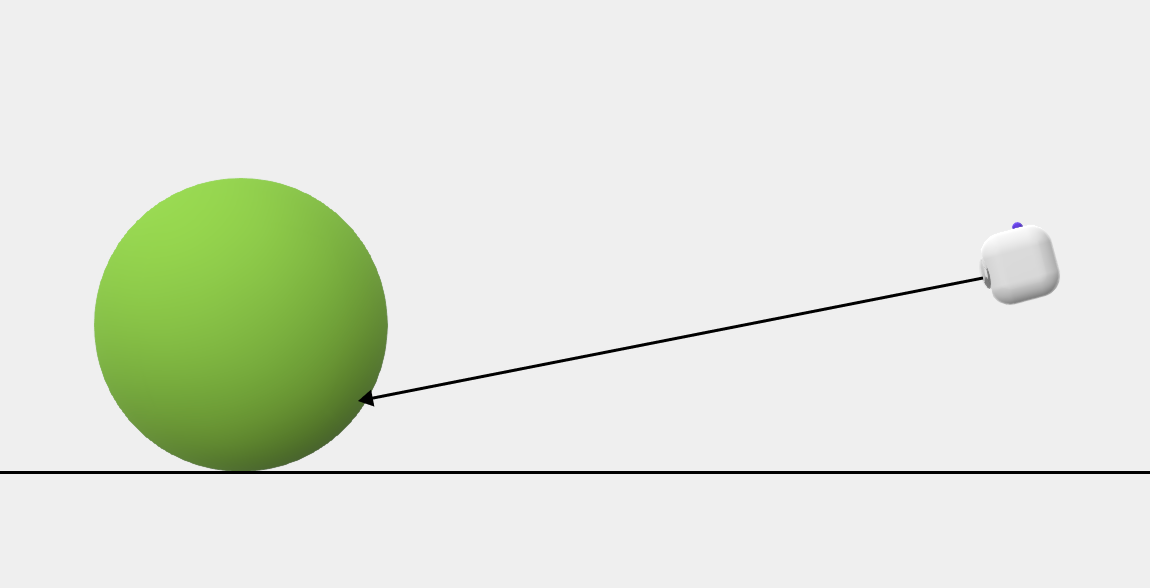
\includegraphics[scale = 0.2]{img/C8/situacion-inicial.png}
    \caption{Situación a la que aplicar Ray-Marching}
    \label{fig:RM-inicial}
\end{figure}

La distancia de un punto $p$ a una esfera $S$ de centro $c$ y radio $r$ es 
\begin{equation}
    \label{eq:distancia-punto-esfera}
    d(p,S) = \|p-c\| - r 
\end{equation}

y la distancia de un punto al plano $y=0$ es simplemente su componente $y$. Por tanto, partiendo del origen, calculamos la distancia a la esfera y la distancia al plano, vemos que es menor la distancia al plano, por lo que avanzamos en el rayo una distancia igual a la distancia que había al plano (imagen \ref{fig:iteraciones-RM} (a)). Seguidamente repetimos la operación: volvemos a calcular la distancia a la esfera y al plano. De nuevo es menor la distancia al plano, por lo que avanzamos en el rayo la misma distancia que había en el plano (imagen \ref{fig:iteraciones-RM} (b)).

\begin{figure}[ht]
    \centering
    \begin{tabular}{ccc}
      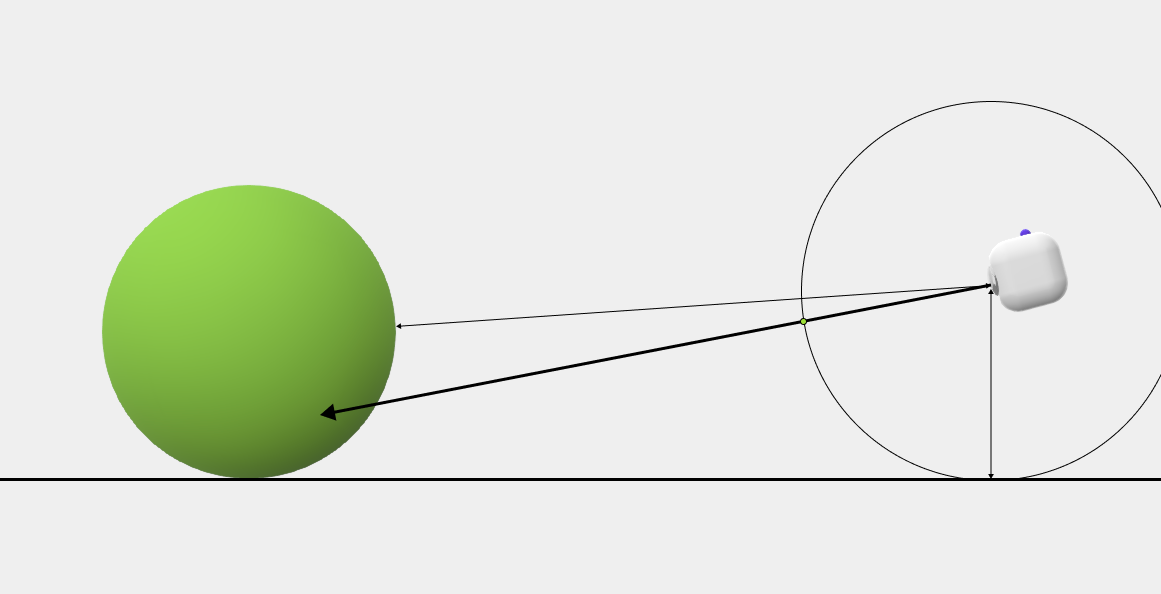
\includegraphics[scale=0.17]{img/C8/ray-marching-1.png} &     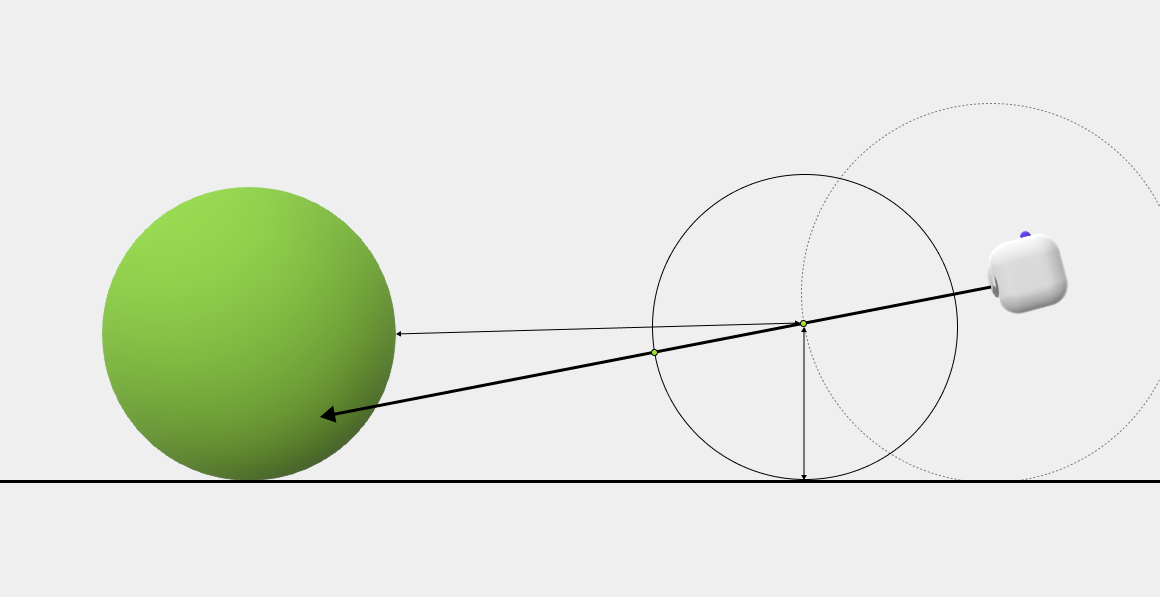
\includegraphics[scale=0.17]{img/C8/ray-marching-2.png} \\
    (a) Primera iteración & (b) Segunda iteración \\[6pt]
    \end{tabular}
    \caption{Dos primeras iteraciones de Ray Marching}
    \label{fig:iteraciones-RM}
\end{figure}

Si repetimos este proceso indefinidamente, llegará el momento en el que la distancia a la esfera será tan pequeña que consideraremos que el punto está en la esfera y habremos encontrado la intersección (imagen \ref{fig:finales} (a)). En caso de que no exista ninguna intersección, el algoritmo seguirá avanzando en el rayo, pero al no intersecar con ninguna superficie se avanzará indefinidamente (imagen \ref{fig:finales} (b)), por lo que hay que fijar una distancia máxima recorrida o un número máximo de iteraciones como parámetro del algoritmo.

\begin{figure}[ht]
    \centering
    \begin{tabular}{ccc}
      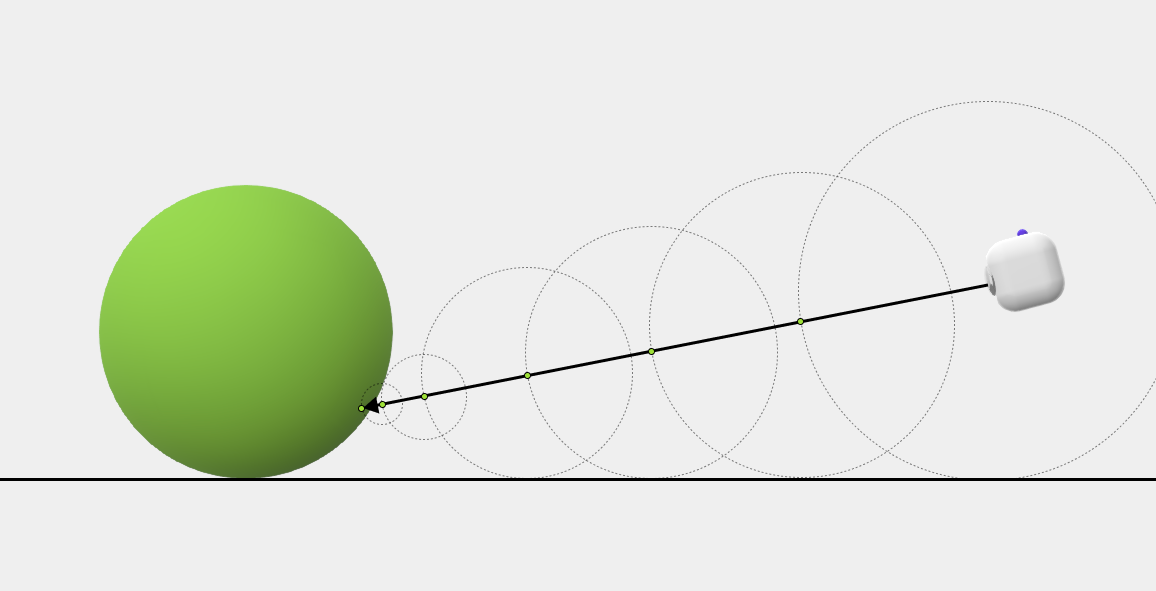
\includegraphics[scale=0.2]{img/C8/ray-marching-final.png} &     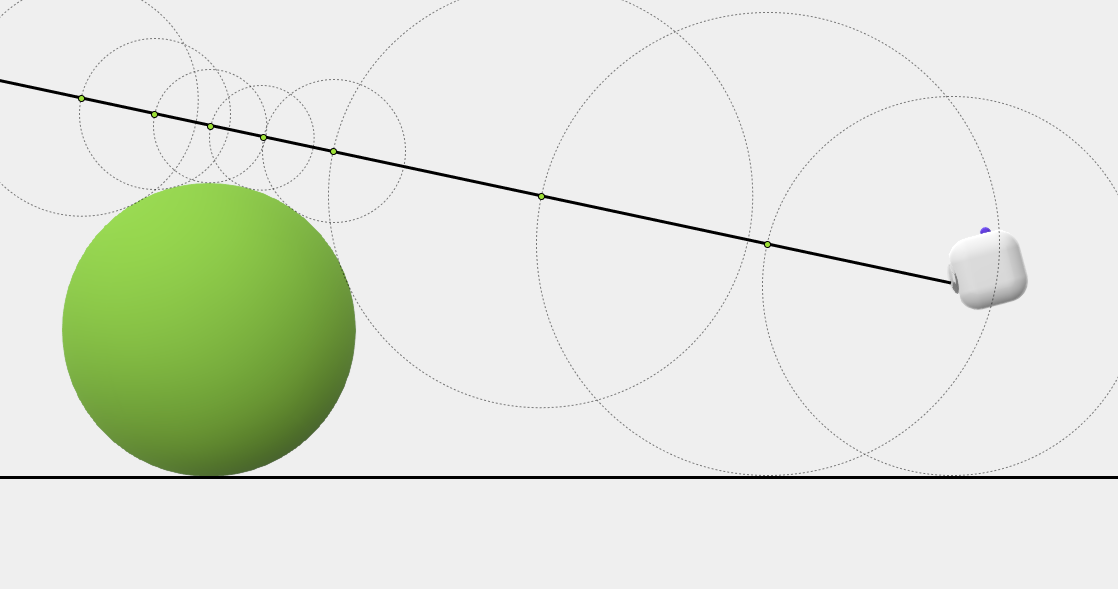
\includegraphics[scale=0.2]{img/C8/ray-marching-miss.png} \\
    (a) Encuentra intersección & (b) El rayo se pierde \\[6pt]
    \end{tabular}
    \caption{Posibles estados finales del algoritmo Ray-Marching}
    \label{fig:finales}
\end{figure}

Por tanto, el algoritmo, si consideramos un conjunto de $objetos$, un rato $R(t)=p_0 + \vec v t$ y un número máximo de avances en el rayo antes de decidir que no existe intersección $MAX\_STEPS$, se describiría como indica el algoritmo \ref{alg:Ray-Marching}.

\begin{algorithm}[H]
\caption{Ray-Marching} \label{alg:Ray-Marching}
%\KwData{Objects: Array de objetos, $\epsilon$: Distancia por debajo de la cual se considera intersección, R: Rayo $R(t)=p_0+\vec v t$}
\begin{algorithmic}
\State $p\gets lookfrom$
\State $steps \gets 0$

\While{$steps < MAX\_STEPS$} \Comment{También se puede fijar una distancia máxima}
    \State $min\_dist \gets MAX\_DIST$
    \State $i\gets 0$

    
    \While{$i < num\_objects$}\Comment{Cálculo de la mínima distancia}
        \State $dist \gets distancia(p, objects[i])$
        \If{$dist < min\_dist$}
            \State $min\_dist \gets dist$
            \State $index\gets i$
        \EndIf
        \State $i++$
    \EndWhile
    \If{$min\_dist < \varepsilon$}
        \State \textbf{Hay intersección} con $objects[index]$
    \Else
        \State $p\gets p + \vec v \cdot min\_dist$ \Comment{Avanzamos en el rayo}
    \EndIf
    \State $steps++$
\EndWhile
\State \textbf{No existe intersección}
\end{algorithmic}
\end{algorithm}

\begin{observacion}
\label{observacion:vector-normalizado}
    Cabe destacar un importante detalle, y es que a partir de este momento es indispensable que en la creación del rayo el vector dirección esté normalizado, pues si queremos avanzar $min\_dist$ unidades en la dirección $\vec v$ y $|v| \not= 1$ se avanzaría una distancia distinta y el algoritmo no funcionaría correctamente.
\end{observacion}

\subsection{Implementación de Ray-Marching en GLSL}

Veámos ahora cómo podemos llevarnos todos estos nuevos conocimientos a la GPU con GLSL. El objetivo ahora es modificar el fragment shader eliminando la dependencia de \verb|Hit_Sphere| y de \verb|Hit_Plane| para utilizar Ray-Marching para calcular las intersecciones. Realmente el resultado de estas modificaciones debería ser el mismo que en el final del capítulo anterior, pero ahora calcularemos las intersecciones de forma distinta. 

Lo primero que necesitaremos es una función que calcule la distancia de un punto a una esfera $S$. Esto es tan sencillo como implementar una función que calcule la fórmula \ref{eq:distancia-punto-esfera}.

\begin{lstlisting}
// Dada una esfera S y un punto p, calcula la distancia
// del punto a la superficie de la esfera
float get_dist_sphere(vec3 p, Sphere S){
    return length(S.center - p) - S.radius;
}
\end{lstlisting}

Por parte del plano, podríamos aprovechar que nuestro plano es el $y=-2$ y simplemente devolver la componente $y$ del punto más dos. Sin embargo, no cuesta tanto calcular la distancia de un punto a un plano arbitrario $Ax+By+Cz = D$, siendo $\vec N=(A,B,C)$ el vector normal al plano. El punto perteneciente a un plano más cercano a otro punto $p$ dado es aquel que interseca con la recta cuyo vector director es el normal al plano y que pasa por $p$. Es decir, el punto de la recta $S(t)=p+\vec Nt$ que satisface la ecuación $(A,B,C)\cdot (x,y,z) = D$. Veámos para qué $t$ se satisfacen las ecuaciones.
\begin{equation}
    \begin{split}
        \vec N\cdot S(t) &= D \\
        \vec N\cdot (p+\vec N t) &= D \\
        t &= \dfrac{D-\vec N \cdot p}{|\vec N|^2}
    \end{split}
\end{equation}
Por tanto la distancia entre punto y plano es la longitud del vector que une a $p$ con $S(t)$, siendo este $t$ el recién calculado. El código entonces sería:
\begin{lstlisting}
// Dado un plano P y un punto p, calcula la distancia del 
// punto p a la superficie del plano.
float get_dist_plane (vec3 p, Plane P) {
    float t_interseccion = (P.D - dot(P.normal,p))/dot(P.normal, P.normal);
    vec3 closest_point = p + t_interseccion * P.normal;
    return length(p-closest_point);
}
\end{lstlisting}

Seguidamente necesitamos fijar dos constantes: el número máximo de iteraciones que se darán en el algoritmo y $\varepsilon$, la distancia mínima por debajo de la misma se considera que un punto pertenece a la superficie. La primera de ellas la podemos tomar como una macro, al igual que hicimos con el tamaño de los arrays, pero la segunda interesa que sea parametrizable, para así poder observar los niveles de detalle y qué variaciones experimenta la escena al modificar este valor. Por ello, usamos una variable \verb|uniform| a la que pasaremos valor vía JavaScript.

\begin{lstlisting}
    uniform float u_epsilon;
    // ... 
    #define MAX_STEPS 1000
\end{lstlisting}

Y ya tenemos todo preparado para implementar el Ray-Marching. La función que dado un rayo calcula posibles intersecciones con los cuerpos y asigna un color en función es \verb|ray_color|, por lo que lo más natural es editar el código de esta función. En lugar de llamar a \verb|hit_sphere_list| y \verb|hit_plane| como hicimos en la sección \ref{subsection:plano} aplicaremos Ray-Marching. Como GLSL no nos permite mantener un array heterogéneo en el que almacenar todos los objetos independientemente de su tipo, tenemos que hacerlo de forma secuencial. Y como tampoco permite acceder a elementos de un array a partir de índices no constantes, utilizaremos una variable donde almacenar la esfera más cercana, para recuperarla en caso de intersección, véase el código.

\begin{lstlisting}
vec4 ray_color(Ray r, Sphere S[ARRAY_TAM], int num_spheres, 
    Plane ground,
    Directional_light lights[ARRAY_TAM], int num_lights) {
    
    Hit_record hr; hr.hit = false;  // Hit_record structure
    float dist = MAX_DIST;          // Distancia a cada objeto 
    vec3 p = r.orig;                // Punto del rayo
    float closest_dist = MAX_DIST;  // Menor distancia
    float current_t = 0.0;          // p=orig+current_t*dir
    vec4 tmp_color;                 // Color temporal
    Sphere S_hit;                   // Esfera mas cercana
    
    int object_index;   // 0,...,num_spheres-1: esferas,
                        // num_spherees: plano
    // Ray Marching
    for(int i = 0; i < MAX_STEPS; i++) {
        // Calculamos el objeto mas cercano
        closest_dist = MAX_DIST;

        // Distancia a las esferas
        for(int i = 0; i < ARRAY_TAM; i++) {
            if(i == num_spheres) break;
            dist = get_dist_sphere(p, S[i]);
            if(dist < closest_dist) {
                closest_dist = dist;
                object_index = i;
                S_hit = S[i];
            }
        }

        // Distancia al suelo
        dist = get_dist_plane(p, ground);
        if(dist < closest_dist) {
            closest_dist = dist;
            object_index = num_spheres;
        }
    
        // closest_dist almacena la menor de las distancias
        // y object_index el indice del objeto mas cercano
        if(closest_dist < u_epsilon){   // Hay interseccion

            hr.hit = true;
            hr.t = current_t;
            hr.p = ray_at(r, hr.t);

            if(object_index == num_spheres){ // Suelo
                // Codigo de interseccion con el suelo ...
            }

            else {      // Una de las esferas
                // Codigo de interseccion con S_hit
            }
        }

        // Si no hay interseccion, avanzamos en el rayo
        current_t += closest_dist;
        p = ray_at(r, current_t);

        // Si estamos muy lejos acabamos el bucle
        if(current_t >= MAX_DIST) break;
    }
    // No hay interseccion
    // Background code ...       
}
\end{lstlisting}

Fíjese que concuerda con la estructura que describe el algoritmo \ref{alg:Ray-Marching}. Hecha esta modificación, el resultado fijando ciertos parámetros dinámicamente es el mostrado en la imagen \ref{fig:esferas-RM}. Tal y como adelantamos, el resultado es igual que cuando calculábamos las intersecciones exactas, ya que realmente lo único que cambia es la forma de calcular las intersecciones, nada estrictamente visual.

\begin{figure} [ht]
    \centering
    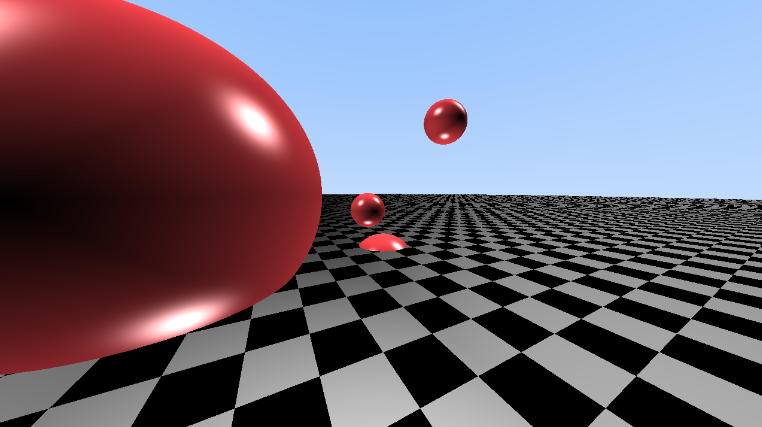
\includegraphics[scale = 0.37]{img/C8/esferas-ray-marching.png}
    \caption{Escena tras implementar Ray-Marching}
    \label{fig:esferas-RM}
\end{figure}

Recordamos e insistimos en que el vector director del rayo \verb|r.dir| debe ser un vector normalizado, es decir, unitario. De otro modo los avances en el rayo no estarán controlados, obsérvese en la imagen \ref{fig:vectores-no-normalizados} los resultados obtenidos al no normalizar el vector director al crear el rayo.

\begin{figure} [ht]
    \centering
    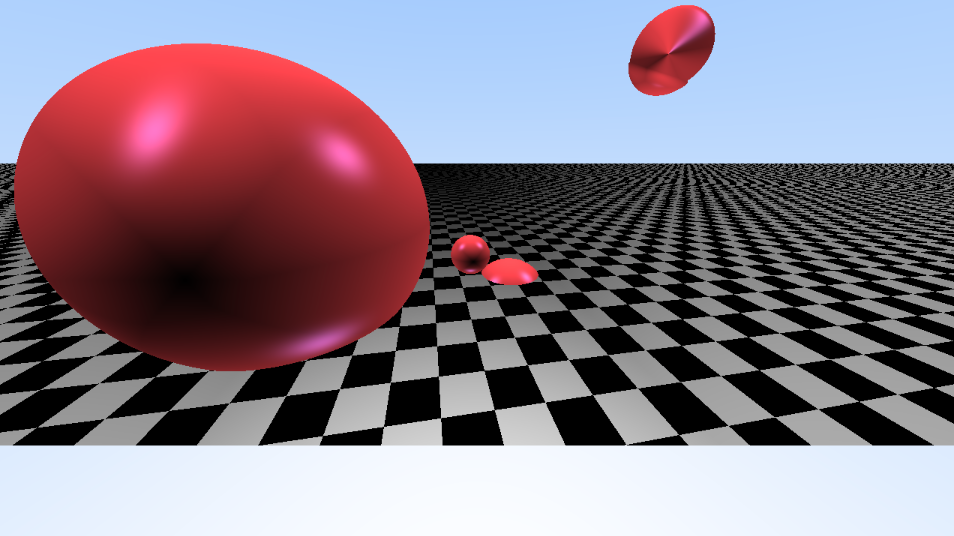
\includegraphics[scale = 0.3]{img/C8/vectores-no-normalizados.png}
    \caption{Escena utilizando vectores no unitarios en los rayos}
    \label{fig:vectores-no-normalizados}
\end{figure}

\subsection{Comentarios sobre Ray-Marching}

Una vez hemos introducido e implementado el algoritmo Ray-Marching, el lector es posible que piense que es una forma menos exacta y además menos eficiente que calcular analíticamente las intersecciones con los cuerpos. Es cierto que en casos como el de esferas o planos cuyas ecuaciones implícitas y sus intersecciones con rayos están muy bien definidos y son sencillas de calcular aplicar ray-marching ralentiza el procesado. Sin embargo muchas superficies, como es el caso de los fractales, no cuentan con una ecuación implícita que la defina. Otras sí cuentan con ecuaciones implícitas pero estas son muy difíciles de resolver. En este último caso se pueden aplicar métodos numéricos para aproximar las soluciones, que son métodos precisamente iterativos. 

Sin embargo, ray-marching sólo necesita, para cada cuerpo, una función que aproxime suficientemente bien la distancia a un conjunto. A partir de un rayo y dichas funciones se puede aplicar ray-marching, de forma que se converge finalmente al punto de intersección. Por contra, si buscamos intersecciones analíticas hay que resolver ecuaciones, en ocasiones para acabar aproximando las soluciones, y retener la más pequeña.

Un aspecto a destacar de ray-marching es la dependencia de sus parámetros. Es importante fijar un valor $\varepsilon$ adecuado, ya que si es demasiado grande puede brindarnos resultados muy pobres. En la imagen \ref{fig:esferas-RM} se ha utilizado $\varepsilon=0.001$ y nos da un resultado muy bueno, pero obsérvese en la imagen \ref{fig:epsilon-grande} qué ocurre si se fija $\varepsilon=0.1$. Los límites de los cuadrados del suelo se distorsionan y las apariencias de las esferas también se ven muy resentidas. Sin embargo es cierto que a mayor valor de $\varepsilon$ menos iteraciones y por tanto más velocidad, pero los resultados son peores. Es por tanto necesario utilizar valores de $\varepsilon$ adecuados a la situación, siendo suficientemente pequeños como para obtener un buen resultado pero suficientemente grandes como para que sea computacionalmente viable.

\begin{figure} [ht]
    \centering
    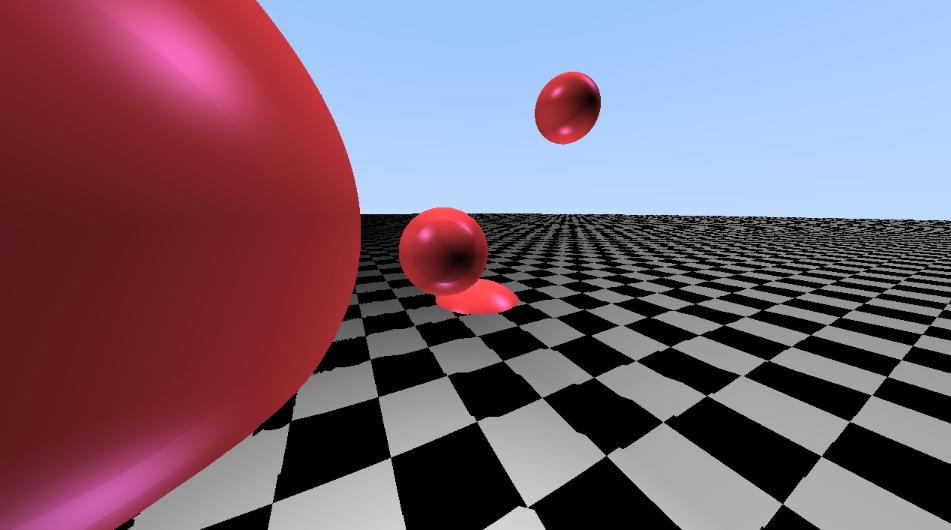
\includegraphics[scale = 0.3]{img/C8/epsilon-grande.png}
    \caption{Escena renderizada utilizando $\varepsilon=0.1$}
    \label{fig:epsilon-grande}
\end{figure}

Una reflexión similar se puede aplicar al parámetro que define el número máximo de iteraciones (\verb|MAX_STEPS|). Pensemos en un rayo que pasa muy cerca de un objeto pero no llega a intersecarlo, sino que finalmente interseca al suelo. Durante las iteraciones que el rayo pase cerca del objeto quizá avance muy lentamente durante varias iteraciones, pues la distancia mínima es la distancia a dicho objeto que es pequeña. Este hecho puede provocar que se alcance el número máximo de iteraciones, considerando así que el rayo no golpea ningún objeto y asignándole el color de fondo cuando realmente con algunas iteraciones más podría alcanzarse la intersección con el suelo. Este hecho se puede observar en la imagen \ref{fig:pocas-iteraciones}, donde se ha utilizado \verb|MAX_STEPS=100|. Fíjese en las fronteras entre el horizonte y las esferas, o en los bordes de las esferas.

\begin{figure} [ht]
    \centering
    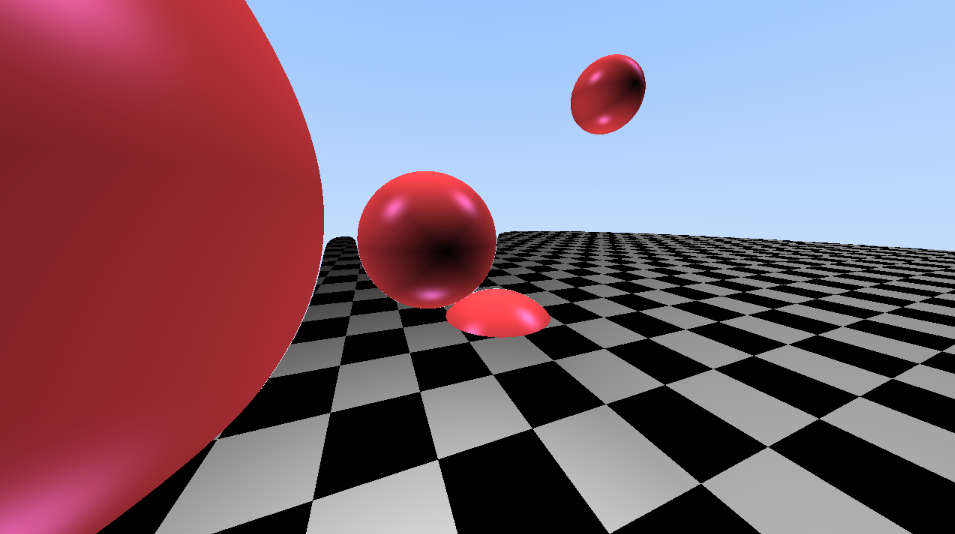
\includegraphics[scale = 0.3]{img/C8/pocas-iteraciones.png}
    \caption{Escena renderizada utilizando MAX\_STEPS=100}
    \label{fig:pocas-iteraciones}
\end{figure}

De igual forma, menos iteraciones implica más rapidez, pero peores resultados, por lo que es necesario fijar un valor correcto.

\section{Signed Distance Functions (SDFs)}
\label{section:SDFs}

Durante toda la sección anterior hemos hablado de que para aplicar ray-marching es necesario que cada objeto que componga la escena cuente con una función que estime la distancia de un punto cualquiera de $\R^3$ a su superficie. En esta sección introduciremos el concepto de SDF y pondremos un ejemplo sencillo con una esfera.

Primero explicaremos brevemente el fundamento matemático. Sea $f:\R^n\longrightarrow\R$ una función continua que define implícitamente el conjunto 
$$
A = \{x\in\R^n: f(x)\leq 0\}.
$$
Por continuidad, $f(x)=0\ \ \forall x\in\partial A$. Decimos que la frontera $\partial A$ define la \textit{superficie implícita} de $f$. De hecho, $f$ es negativa en el interior de $A$ ($f(x)<0 \ \ \forall x\in\mathring A$), por lo que podemos decir que dicha superficie implícita $\partial A$ coincide precisamente con el conjunto $f^{-1}(0)$. A partir de una función real y continua podemos entonces definir una superficie en $\R^n$.

\begin{definicion}[SDF]
    Una función continua $f:\R^3\longrightarrow\R$ se conoce como una \textbf{`Signed Distance Bound'} (cota de la distancia con signo) de su superficie implícita $f^{-1}(0)$ si, y solo si
    \begin{equation}
        \label{eq:SDB}
        |f(x)|\leq d(x,f^{-1}(0)) \ \ \forall x\in\R^3
    \end{equation}
    
    Si se tiene la igualdad en (\ref{eq:SDB}), entonces $f$ es una \textbf{`Signed Distance Function'} (función distancia con signo).
\end{definicion}

Una forma sencilla de entender este concepto es concibiendo una superficie como los puntos en los que se anula la función distancia. Es decir, si un punto se sitúa a distancia 0 es porque pertenece a dicha superficie. En caso de que la distancia sea positiva en módulo el punto se sitúa fuera, tan lejos como diga dicho módulo.

Como ya hemos visto en la sección anterior, algunas primitivas, como las esferas, pueden ser fácilmente definidas por su SDF. Recordamos que la SDF de una esfera es $f(x)=|x-c|-r$ siendo $c\in\R^3$ su centro y $r\in\R$ su radio. Entonces un punto exterior a la esfera tendrá un valor de la SDF positivo, uno interior tendrá un valor negativo y únicamente se anulará en el caso de que el punto pertenezca a la superficie de la esfera (ver imagen \ref{fig:SDF-esfera}). En \cite[Table 1]{Hart-1995} podemos encontrar una lista de primitivas con referencias a sus correspondientes SDFs.

\begin{figure} [ht]
    \centering
    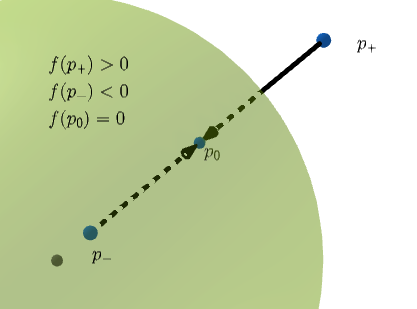
\includegraphics[scale = 0.5]{img/C8/SDF-esfera.png}
    \caption{Ejemplos de puntos con distintos valores de la SDF de una esfera}
    \label{fig:SDF-esfera}
\end{figure}

\section{Visualización tridimensional de conjuntos de Julia}

Una vez tenemos definido el algoritmo que usaremos para la visualización de fractales, que es el algortimo de ray-marching acompañado de una SDF concreta, es momento de trabajar en la visualización de fractales 3D. Comenzaremos, siguiendo el mismo orden que adoptamos en el capítulo \ref{chap:fractales-2D}, por los conjuntos de Julia en 3D.

Recordemos de la sección \ref{section:Julia} que el conjunto de Julia $\mathcal{J}_c$ de un número complejo fijo $c\in\C$ se define como la frontera entre el conjunto de puntos prisioneros y el conjunto de puntos de escape bajo la iteración de la función $P_{c}(z)=z^2+c$. Es decir, $\mathcal{J}_c = \partial \mathsf{E}_c$, donde
\begin{equation}
    \mathsf{E}_c = \{z_0\in\C: \{|P_c^n(z_0)|\}\rightarrow \infty \}
\end{equation}

Queda por tanto a la vista una clara dependencia de los números complejos en esta definición, los cuales podemos identificar únicamente con puntos del plano euclídeo $\R^2$. Necesitamos por tanto una generalización tridimensional de los números complejos. Estrictamente, no existe como tal una generalización tridimensional que mantenga la aritmética compleja, pero sí que existe una en cuatro dimensiones: los cuaternios, usualmente denotados como $\H$.

Podemos encontrar información sobre los cuaternios en \cite{quaternions}, pero introduciremos brevemente su aritmética. De igual forma que para los números complejos se utiliza la unidad imaginaria $i$, en los cuaternios se tienen tres unidades imaginarias: $i,j,k$, de tal manera que un cuaternio se compone de una parte real y tres imaginarias, pudiendo expresarlo como:
\begin{equation}
    q = x\cdot i + y\cdot j + z \cdot k + w \cong (x,y,z,w)\in \R^4.
\end{equation}

Nótese que estamos denotando como componente real a $w$, la última de la terna $(x,y,z,w)$. Las unidades imaginarias se multiplican entre ellas siguiendo las siguien reglas:
\begin{equation}
    \label{eq:relaciones-cuaternios}
    \begin{split}
        ij = k \quad jk &= i \quad ki = j \\
        ji = -k \quad kj &= -i \quad ik = -j \\
        i^2 = j^2 &= k^2 = -1. 
    \end{split}
\end{equation}

Lo cual nos da a entender que los cuaternios tienen estructura de anillo no conmutativo. Una forma de calcular el producto de dos cuaternios arbitrarios $q = q_x\cdot i + q_y\cdot j + q_z \cdot k + q_w\cong (q_x,q_y,q_z,q_w)$ y $q' = q'_x\cdot i + q'_y\cdot j + q'_z \cdot k + q'_w\cong (q'_x,q'_y,q'_z,q'_w)$ es expandiendo la expresión

\begin{equation}
    qq' = (q_x\cdot i + q_y\cdot j + q_z \cdot k + q_w)(q'_x\cdot i + q'_y\cdot j + q'_z \cdot k + q'_w) 
\end{equation}

Si utilizamos su expresión como ternas de $\R^4$, denotando $q=(q_{xyz},q_w), q'=(q'_{xyz},q_w)$, agrupando términos y aplicando las relaciones \ref{eq:relaciones-cuaternios} el resultado puede expresarse mediante productos vectoriales y escalares:
\begin{equation}
    \label{eq:producto-cuaternios}
    \begin{split}
        (qq')_{xyz} &= q_{xyz}\times q'_{xyz} + q_w q'_{xyz} + q'_wq_{xyz} \\
        (qq)_w &= q_wq'_w - (q_{xyz}\cdot q'_{xyz})
    \end{split}
\end{equation}

Aplicando estas relaciones podemos deducir el cuadrado de un cuaternio con tan solo multiplicar un cuaternio $q$ por sí mismo, obteniendo

\begin{equation}
    \label{eq:cuadrado-cuaternio}
    \begin{split}
        (q^2)_{xyz} &= 2q_w q_{xyz} \\
        (q^2)_w &= q_w^2 - q_{xyz}\cdot q_{xyz},
    \end{split}
\end{equation}
que realmente es una simplificación de las ecuaciones (\ref{eq:producto-cuaternios}) teniendo en cuenta que el producto vectorial de un vector por sí mismo es $0$.

Y una vez tenemos clara la aritmética básica de los cuaternios, podemos generalizar fácilmente los conjuntos de Julia sin más que extender la función $P_c(z)$ a $\H$, fijando un cuaternio $c\in\H$:
\begin{equation}
    \label{eq:f-julia-cuaternios}
    \begin{split}
        P_c :& \H \longrightarrow \H \\
        q & \longmapsto q^2 + c
    \end{split}
\end{equation}

De forma que ahora separamos el espacio $\H$ en puntos prisioneros y de escape frente a la iteración de $P_c(q)$ y redefinimos los conjuntos de Julia en 4D como la frontera entre los puntos prisioneros y de escape. 

Sin embargo, es claro que no podemos visualizar conjuntos en 4D de forma tan directa como lo hacemos en 2D, pero sí podemos generarlos y visualizar una proyección en 3D. Pensemos en los mapas de curvas de nivel que se usan en topografía (imagen \ref{fig:curva-de-nivel}), los cuales fijando una altura concreta representan la curva que dibujaría una montaña al intersecarla con un plano horizontal situado a esa altura, permitiéndonos hacernos una idea de la forma en 3D de la montaña a partir de un plano en 2D. 

\begin{figure} [ht]
    \centering
    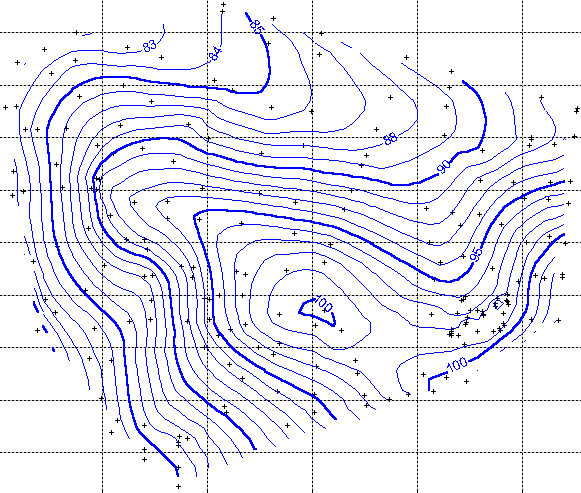
\includegraphics[scale = 0.3]{img/C8/curvas-de-nivel2.png}
    \caption{Representación de una montaña con curvas de nivel}
    \label{fig:curva-de-nivel}
\end{figure}

En nuestro contexto, podemos fijar una dimensión y visualizar el conjunto de Julia para las otras tres, pudiendo modificar después la dimensión que hemos fijado. 

Es por tanto momento de estimar la distancia de un punto cualquiera $p\in\R^3$ a un conjunto de Julia $\mathcal{J}_c$, con $c\in\H$. Lo primero es indentificar un punto del espacio euclídeo $(x,y,z)\in\R^3$ con un cuaternio. La manera más natural es identificar $x$ con la parte real y la segunda y tercera componente con las dos primeras componentes imaginarias. Es decir,
\begin{equation}
    p=(x,y,z)\cong q = x + yi + zj \cong (y,z,0,x)
\end{equation}
Tengamos en cuenta que en principio los rayos van a partir de un punto que está fuera del conjunto de Julia, es decir, al iterar la función $P_c$ la sucesión va a ser divergente, por lo que la SDF nos debe de dar una distancia positiva. La idea es que cada vez nos dé un valor menor conforme nos acerquemos a $\mathcal{J}_c$ hasta prácticamente anularse en caso de que el rayo interseque con el conjunto. 

Debemos por tanto antes de nada iterar $q$ para hacernos a la idea de esta distancia al conjunto, de forma que si tras cierto número $M$ de iteraciones el módulo de la iterada $|P_c^M(q)|$ no es suficientemente grande consideraremos que el punto es convergente, aunque esto probablemente nunca ocurra durante el proceso de ray-marching, pues se evaluarán puntos que están en el conjunto de puntos de escape, en búsqueda de esta frontera. Es decir, iteramos el punto con una amplia posibilidad de que antes o después la $n$-ésima iterada tenga un módulo grande. Denotamos como $q_n=P_c^n(q)$ a esta $n$-ésima iterada. A partir de este valor, definimos la SDF del conjunto de Julia como 
\begin{equation}
    \label{eq:SDF-Julia}
    \begin{split}
        d_c&:\R^3\longrightarrow\R \\
        d_c(p) &= \dfrac{|q_n|\log|q_n|}{2|q'_n|}
    \end{split}
\end{equation}

donde $q'_n$ es otra sucesión iterativa que se puede calcular conjuntamente con $q_n$ mediante $q'_{i+1}=2q_i q'_i$, comenzando con $q'_0=1\cong(0,0,0,1)$, aunque como realmente sólo necesitamos su módulo podemos calcular $|q'_{i+1}|=2|q_i||q'_i|$. Intuitivamente, fíjese que realmente es una forma iterativa de aplicar la derivada de (\ref{eq:f-julia-cuaternios})

Es difícil explicar y entender la génesis de esta fórmula, aunque los detalles matemáticos concretos pueden encontrarse en \cite[Capítulo 8]{Hubbard-Douady}. 

Es decir, iterando el punto inicial y aplicando la transformación (\ref{eq:SDF-Julia}) podemos estimar a qué distancia se sitúa el punto del conjunto de Julia $\mathcal{J}_c$.

\subsection{Aproximando la normal}

Teniendo esta estimación de la distancia podemos calcular el posible punto de intersección de un rayp con $\mathcal{J}_c$, pero si queremos evaluar el modelo de iluminación en dicho punto, antes necesitamos conocer la normal a la superficie en dicho punto. Y aquí es donde tenemos que afrontar la dificultad que supone la propia belleza de los fractales, que es su irregularidad y que su superficie en general no es diferenciable. No existen formas de calcular de forma exacta esta normal, pero en realidad nosotros estamos fijando una resolución que limita el nivel de detalle de la figura, por lo que podemos utilizar ciertos métodos para aproximar esta normal.

\subsubsection{Método 1: Gradiente de la SDF}

La manera más sencilla de obtener un vector normal a la superficie es tomando el gradiente de la SDF, el cual evidentemente no calculamos analítica sino numéricamente utilizando diferencias centradas. Para ello, fijado un punto $p\in\R^3$, calculamos 6 puntos muy próximos a él, sumando y restando en cada una de sus tres componentes un pequeño incremento, que por simplicidad consideraremos que será el propio $\varepsilon$ que fijamos al hacer ray-marching. En cada uno de los 6 puntos evaluamos la SDF y calculamos para cada componente la diferencia, tomando como normal el vector formado por cada una de estas diferencias divididas normalizado.

\begin{algorithm}[H]
    \caption{Cálculo de la normal mediante el gradiente de la SDF} \label{alg:normal-gradiente-sdf}
    \begin{algorithmic}
    \State $h\gets\varepsilon$
    \State $g_{x+}\gets p + (h,0,0)$
    \State $g_{x-}\gets p - (h,0,0)$
    \State $g_{y+}\gets p + (0,h,0)$
    \State $g_{y-}\gets p - (0,h,0)$
    \State $g_{z+}\gets p + (0,0,h)$
    \State $g_{z-}\gets p - (0,0,h)$

    \State $\nabla d_{c_x} \gets d_c(g_{x+})-d_c(g_{x-})$
    \State $\nabla d_{c_y} \gets d_c(g_{y+})-d_c(g_{y-})$
    \State $\nabla d_{c_z} \gets d_c(g_{z+})-d_c(g_{z-})$
        \State \textbf{return} $\dfrac{(\nabla d_{c_x},\nabla d_{c_y},\nabla d_{c_z})}{\|(\nabla d_{c_x},\nabla d_{c_y},\nabla d_{c_z})\|}$
    \end{algorithmic}
\end{algorithm}

En realidad debería tomarse en cada componente del gradiente la diferencia dividida entre $2h$, pero la propia normalización del vector se encarga de reescalar el vector adecuadamente.    

\subsubsection{Método 2: Técnica del tetraedro}

Consideramos un tetraedro cuyos vértices son $k_0=(1,-1,-1)$, $k_1=(-1,-1,1)$, $k_2=(-1,1,-1)$ y $k_3=(1,1,1)$. Sean ahora los puntos $p_i := p+\varepsilon k_i\ \ i=0,\dots,3$. Entonces la normal a la superficie en el punto $p$ es la normalización del vector $\sum_{i=0}^3 k_i d_c(p_i)$. Consúltese \cite{normals-sdf} si se desea tener una justificación del funcionamiento de este método.

\begin{algorithm}[H]
    \caption{Técnica del tetraedro para el cálculo de normales} \label{alg:normal-tetraedro}
    \begin{algorithmic}
    \State $h\gets\varepsilon$
    \State $p_0 \gets p + h(1,-1,-1)$
    \State $p_1 \gets p + h(-1,-1,1)$
    \State $p_2 \gets p + h(-1,1,-1)$
    \State $p_3 \gets p + h(1,1,1)$

    \State $N\gets \sum_{i=0}^3 k_i d_c(p_i)$

    \State \textbf{return} $\dfrac{N}{\|N\|}$
    \end{algorithmic}
\end{algorithm}

\subsection{Implementación en GLSL}

Tenemos por tanto ya la forma de calcular tanto la distancia de un punto al conjunto de Julia de un $c\in\H$ fijo como un método para calcular la normal a la superficie del fractal en un punto, dos de hecho. Es por tanto momento de la implementación. Basta con programar funciones que calculen la SDF y sustituir las llamadas a \verb|get_dist_sphere| por una llamada a dicha función, y una vez se conoce el punto de intersección calcular la normal y evaluar el modelo de iluminación.

De manera natural, igual que identificamos un cuaternio con un elemento de $\R^4$ utilizaremos el tipo \verb|vec4| para representar a los mismos en GLSL. Recordemos que en este caso es la última componente la parte real del cuaternio.

\begin{lstlisting}
vec4 q; // Representa un cuaternio (x,y,z,w)
// q = xi + yj + zk + w
\end{lstlisting}

Si ahora seguimos la ecuación (\ref{eq:cuadrado-cuaternio}) podemos rápidamente implementar una función que dado un cuaternio calcule su cuadrado.

\begin{lstlisting}
// Dado un cuaternio q, calcula su cuadrado q^2
vec4 quat_square(vec4 q){
    vec3 xyz = 2.0*q.w*q.xyz;
    float w = q.w*q.w - dot(q.xyz, q.xyz);
    return vec4(xyz, w);
}
\end{lstlisting}

Por lo que gracias a esta función y a la aritmética ya programada es sencillo programar la función $P_c(q)=q^2+c$. Utilizamos una función para iterar el cuaternio asociado a un punto $p$, aprovechando la posibilidad que nos ofrece GLSL de simular el paso de parámetros por referencia mediante las variables \verb|out| e \verb|inout|. En el último caso, una función recibe un parámetro y en caso de que su valor cambie éste mantiene su valor tras el retorno de la función. El código de la función es 
\begin{lstlisting}
// Itera la funcion P_c y obtiene tanto q_n como |q'_n|
// q: Cuaternio que se itera
// dq: Sucesion |q'_n|
// c: Constante fija de P_c asociada al conjunto de Julia
void iterate_julia(inout vec4 q, inout float dq, vec4 c) {
    for(int i = 0; i < MAX_STEPS; i++) {
        dq = 2.0 * length(q) * dq;
        q = quat_square(q) + c;     // P_c(q) = q^2 +c
        if(dot(q, q) > 256.0) break;    // |q| es grande
    }
}
\end{lstlisting}

Fíjese que esta función itera un cuaternio mediante la función $P_c(q)$ y a la vez calcula la sucesión recurrente $|q'_{i+1}|=2|q_n||q'_n|$. Por tanto, el cálculo de la distancia de un punto $p$ al conjunto $\mathcal{J}_c$ se reduce a identificar $p\in\R^3$ con un cuaternio $q\in\H$, iterar $q$ y $|q'|$ teniendo en cuenta que la iteración de $q'$ comienza en $1$ y aplicar la función (\ref{eq:SDF-Julia}).

\begin{lstlisting}
float get_dist_julia(vec3 p, vec4 c) {
    float dist;
    vec4 q = vec4(p.y, p.z, 0.0, p.x);
    float dq = 1.0;     // q'_0 = 1
    iterate_julia(q, dq, c);
    float length_q = length(q);
    return 0.5*length_q * log(length_q) / dq;
}
\end{lstlisting}

Y ya tenemos implementada la SDF de Julia. únicamente resta un método para calcular normales. Como hemos presentado dos, implementaremos los dos, utilizando ahora compilación condicional mediante macros para decidir cuál emplear. Tan solo tenemos que implementar los algoritmos \ref{alg:normal-gradiente-sdf} y \ref{alg:normal-tetraedro}. % TODO Seguimos con esto?

\begin{lstlisting}
// Calcula la normal al conjunto J_c en el punto p
vec3 calculate_normal_julia(vec3 p, vec4 c) {
    vec3 N;
    float h = u_epsilon;

    #if NORMAL == 0
    // Gradiente de la SDF
    vec4 qp = vec4(p.y, p.z, 0.0, p.x);
    float gradX, gradY, gradZ;
    vec3 gx1 = (qp - vec4( 0.0, 0.0, 0.0, h )).wxy;
    vec3 gx2 = (qp + vec4( 0.0, 0.0, 0.0, h )).wxy;
    vec3 gy1 = (qp - vec4( h, 0.0, 0.0, 0.0 )).wxy;
    vec3 gy2 = (qp + vec4( h, 0.0, 0.0, 0.0 )).wxy;
    vec3 gz1 = (qp - vec4( 0.0, h, 0.0, 0.0 )).wxy;
    vec3 gz2 = (qp + vec4( 0.0, h, 0.0, 0.0 )).wxy;
    
    gradX = (get_dist_julia(gx2,c) - get_dist_julia(gx1,c))/(2.0*h);
    gradY = (get_dist_julia(gy2,c) - get_dist_julia(gy1,c))/(2.0*h);
    gradZ = (get_dist_julia(gz2,c) - get_dist_julia(gz1,c))/(2.0*h);
    N = normalize(vec3( gradX, gradY, gradZ ));

    #else
    // Metodo del tetraedro
    const vec2 k = vec2(1,-1);
    N = normalize( k.xyy*get_dist_julia( p + k.xyy*h, c ) + 
                   k.yyx*get_dist_julia( p + k.yyx*h, c ) + 
                   k.yxy*get_dist_julia( p + k.yxy*h, c ) + 
                   k.xxx*get_dist_julia( p + k.xxx*h, c ) );

    #endif
    return N;
}
\end{lstlisting}

Y ya únicamente resta sustituir en el ray-marching las SDFs y el método para calcular normales de las esferas por el código que corresponde a los conjuntos de Julia. Para poder dinamizar el cuaternio $c\in\H$ que se considera fijo en los cálculos declaramos una variable \verb|uniform| al igual que se hizo a la hora de los conjuntos de Julia 2D. También creamos una variable global que es \verb|Material fractal_material;| que como su propio nombre indica es el material que se le asignará al objeto fractal.

\begin{lstlisting}
// Cuaternio c fijo. Visualizaremos el conjunto J_c
uniform vec4 u_julia_set_constant;
// Material que se asigna al fractal
Material fractal_material
// ...

vec4 ray_color(Ray r, Plane ground, 
    Directional_light lights[ARRAY_TAM], int num_lights) {

    // ... 
    int object_index; // 0: Ground, 1: Julia

    // Ray Marching
    for(int i = 0; i < MAX_STEPS; i++) {
        closest_dist = MAX_DIST;
        // Distancia al plano
        dist = get_dist_plane(p, ground);
        if(dist < closest_dist) {
            closest_dist = dist;
            object_index = 0;
        }
        // Distancia a Julia
        dist = get_dist_julia(p , u_julia_set_constant);
        if(dist < closest_dist){
            closest_dist = dist;
            object_index = 1;
        }

        if(closest_dist < u_epsilon){   // Hay interseccion
            hr.hit = true;
            hr.t = current_t;
            hr.p = ray_at(r, hr.t);
            if(object_index == 0){      // r hits the ground
                // ... 
            else {      // r hits Julia
                hr.mat = fractal_material;
                hr.normal = calculate_normal_julia(
                    hr.p, u_julia_set_constant);
            return evaluate_lighting_model(lights, num_lights, hr);
        }
        current_t += closest_dist;
        p = ray_at(r, current_t);
        if(current_t >= MAX_DIST) break;
    }
    // r does not hit nothing
    // ... 
}
\end{lstlisting}

Y con esta modificación de \verb|ray_color| podemos ya visualizar conjuntos de Julia tridimensionales. Podemos también cambiar los parámetros del material para observar distintas apariencias. 

En las imágenes \ref{fig:julia-3D} podemos ver algunos de los resultados que, después de este largo camino, hemos podido obtener modificando los parámetros.

\begin{figure}[ht]
    \centering
    \begin{tabular}{cc}
      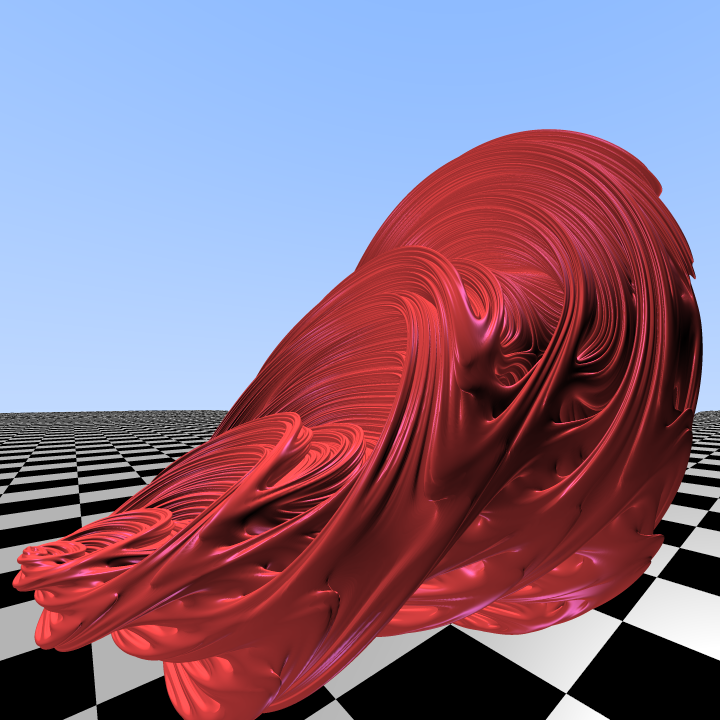
\includegraphics[scale=0.28]{img/C8/julia-1.png} &     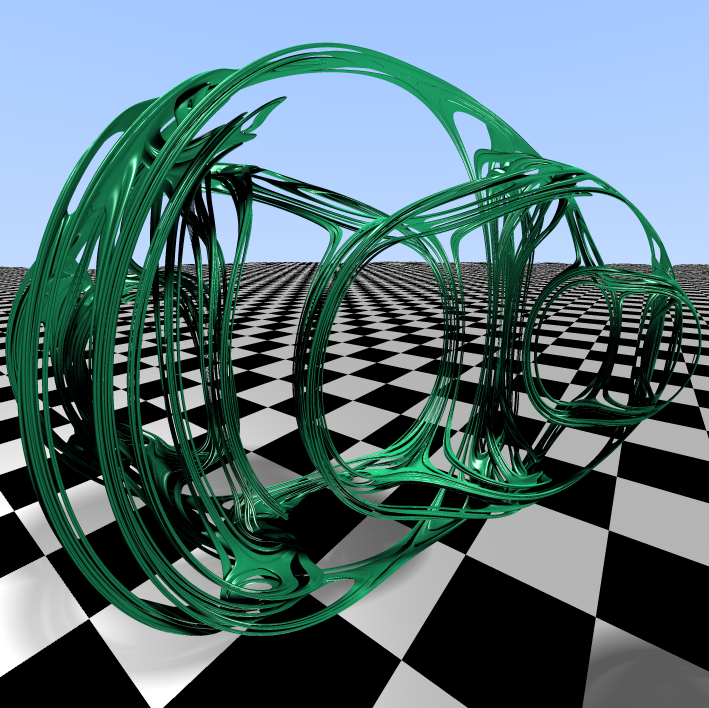
\includegraphics[scale=0.36]{img/C8/julia-2.png} \\
    (a) $c=-0.12+0.75 i$ & (b) $c=0.3+1.09j+0.3k$ \\[6pt]
    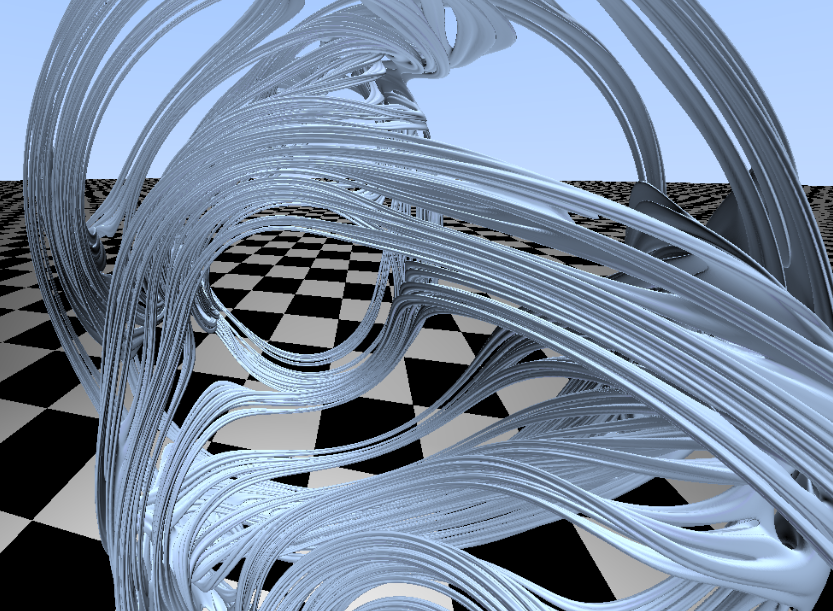
\includegraphics[scale=0.21]{img/C8/julia-3.png} &     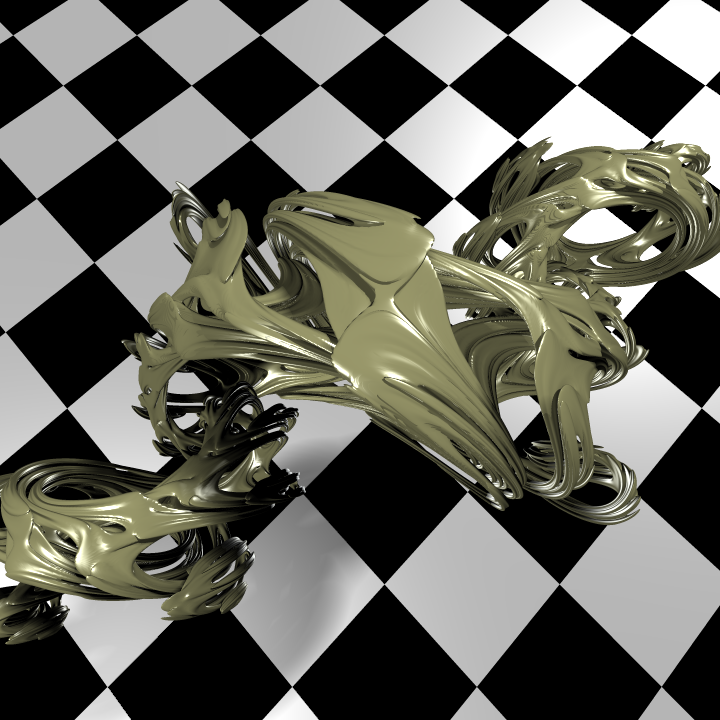
\includegraphics[scale=0.25]{img/C8/julia-4.png} \\
    (c) $c=0.1+0.74i+0.62j+0.14k$ & (d) $c=-0.81-0.48j-0.1k$ \\[6pt]
    \end{tabular}
    \caption{Conjuntos de Julia 3D para distintos $c\in\H$}
    \label{fig:julia-3D}
\end{figure}

